%Archivo latex del proyecto final

%Formato artículo, tamaño de letra 11
\documentclass[11pt,a4paper]{article}


%Todos estos paquetes son los que he usado en el tfg
%Sé que hay muchos, pero por si acaso los pongo
\usepackage[utf8x]{inputenc}
\usepackage{array}
\usepackage{amsmath}
\usepackage{amsbsy}
\usepackage{bm} %Para poner en negrita las letras griegas, tambien sirve el de arriba
\usepackage{upgreek} %Para quitarle la cursiva a las letras griegas, con el comando \up''letra griega'' todo junto
\usepackage{mathrsfs} 
\usepackage{amssymb}
\usepackage{marvosym}
\usepackage{epsfig}
\usepackage{graphics}
\usepackage{graphicx}
\usepackage{amsfonts}
\usepackage{xspace}
\usepackage{color}
\usepackage{booktabs}
\usepackage{xtab}
\usepackage{subfig}
\usepackage{graphicx}

\usepackage[spanish]{babel}

\begin{document}

\title{\'Atomos Ultrafr\'ios}
\author{Jos\'e Ponce Chulani}

\maketitle


\bigskip

\begin{abstract}
  %URL del repositorio
  En este artículo vamos a tratar brevemente un campo de la física cuántica que está en auge: el de los \'atomos y m\'oleculas ultrafr\'ias. Nos centraremos en el modelo de Bose-Hubbard para estudiar algunas de sus propiedades.
\end{abstract}

\bigskip

\textit{Palabras Clave:}
Átomos ultrafríos, modelo Bose-Hubbard, superfluido, aislante Mott, tuneleo.

 

\begin{abstract}
  %URL del repositorio
  In the current proyect we give a brief review of an investigation field of quantum physics that is very popular nowadays: the ultracold atoms or molecules. Specifically we study some properties of the Bose-Hubbard model. 
\end{abstract}

\bigskip

\textit{Keywords:}
Ultracold atoms, Bose-Hubbard model, suprfluid, Mott insulattor, tunneling.



\section{Introducción}


\section{El sistema}

Como ya hemos mencionado nuestro modelo contiene dos ingredientes básicos: una red óptica y una cierta cantidad de átomos que vamos a cargar en la red. Estos átomos van a ser de carácter bosónico, de manera que tendremos la libertad de almacenar tantos como queramos (o cuanto podamos, mejor dicho) en un mismo estado cuántico. La dinámica de los bosones a lo largo de la red va a depender de dos términos fundamentalmente, la energía cinética de los átomos y de cuán fuerte interaccionen entre ellos, pudiendo dar lugar al famoso efecto túnel cuando la primera energía domine sobre la otra.



La red óptica se logra haciendo interferir dos rayos láser, formando un patrón de pozos potenciales. En este patron se carga el gas de bosones ya enfriado, de manera que un esquema del sistema viene dado por la figura \ref{f:red}.

\begin{figure}[h]
  \centering
  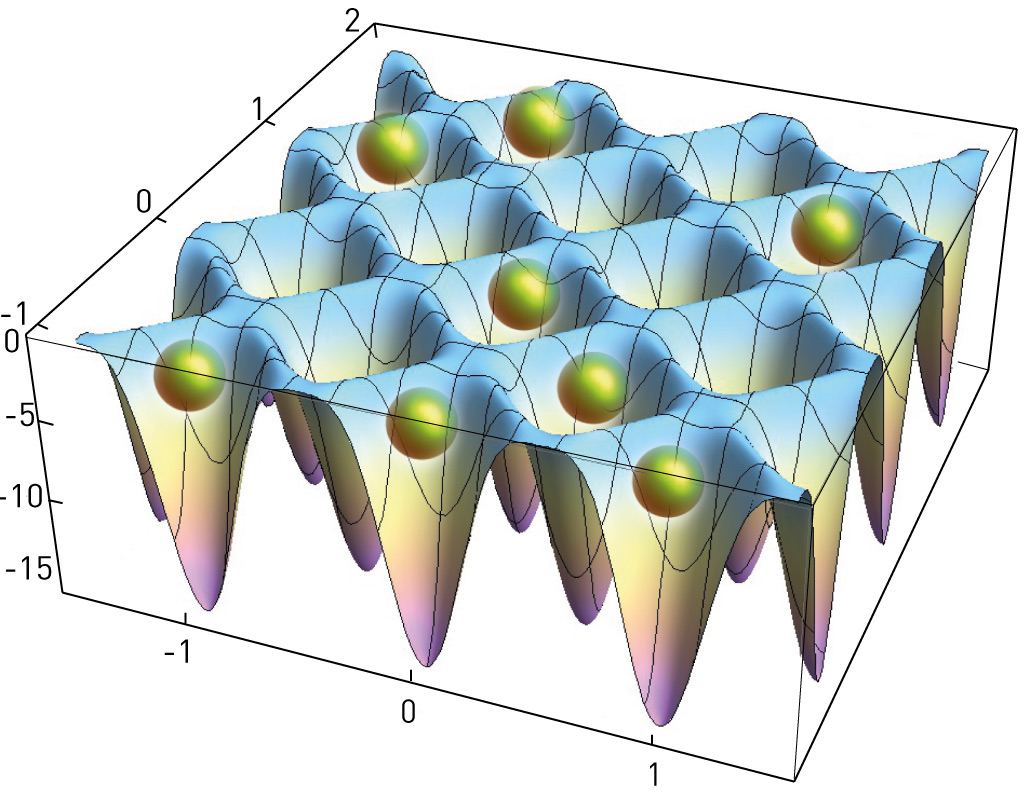
\includegraphics[width=8cm]{hi_8148.jpg}
  \caption{Esquema de una red óptica bidimensional con átomos en sus pozos potenciales.}
  \label{f:red}
\end{figure}
\noindent

De esta figura también puede verse que es el mismo concepto que las redes cristalinas en física del estado sólido. Por tanto, usaremos las funciones de Bloch para describir a nuestros bosones descolalizados en la red, recordemos que, para un espaciado de la red $a$, las soluciones de la ecuación de Schroedinger vienen dadas por

\begin{equation}
  \begin{split}
    & \phi^{(n)}(x)=\textit{e}^{iqx}u_q^{(n)}(x) \\
    & u_q^{(n)}(x+a)=u_q^{(n)}
  \end{split}
\end{equation}

donde q es el número de onda de la partícula y $u_q^{(n)}(x)$ es la función que contiene la perioricidad de la solución.



A partir de estas funciones se definen las conocidas funciones de Wannier, que se usan para localizar los átomos en un mínimo de potencial dado. Estas funciones se definen:

\begin{equation}
  \omega_n(x-x_j)=\frac{1}{\sqrt{N_L}}\sum_q\textit{e}^{-iqx_j}\phi_q^{(n)}(x)
\end{equation}


\subsection{Modelo Bose-Hubbard}

Aquí vamos a hacer una breve derivación del Hamiltoniano Bose-Hubbard. Si suponemos que la red tiene un potencial $V_{lattice}(x)$ y nuestra función de onda $\psi(x)$, entonces el Hamiltoniano de un gas de bosones fríos viene dado por

\begin{equation}
  \begin{split}
    H = & \int d³x \phi^{\dagger}(x)(-\frac{\hbar^2}{2m}\nabla^2+V_{lattice}(x))\phi(x)+\int d³x\phi^{\dagger}(x)(V_T(x)-\mu) \\
    &-\frac{g}{2}\int d³x\phi^{\dagger}\phi^{\dagger}\phi\phi
  \end{split}
\end{equation}

donde $V_T(x)$ es el potencial que atrapa el gas de bosones y $g$ es la interacción de partículas en un mismo pozo potencial.



Haciendo algunas suposiciones como que los bosones solamente interaccionan a traves de onda $s$, y solamente dejando tunelear entre vecinos más próximos se puede llegar al Hamiltoniano simplificado


\begin{equation}
  H=-J\sum_{\langle i,j\rangle}b_i^{\dagger}b_j+\frac{U}{2}\sum_iN_i(N_i-1)-\mu\sum_iN_i
\end{equation}

donde $b_i$ ($b_i^{\dagger}$) es el operador destrucción (creación) de un bosón en el sitio $i-$\'esimo a partir de los cuales se define el operador número $N_i=b_i^{\dagger}b_i$.

A partir de esta ecuación solamente tenemos que darle valores números a $J$ y $U$ (términos correspondientes al tuneleo e interacción entre partículas) para estudiar la dinámica de nuestro sistema.


Por último mencionar que aquí estudiaremos el caso con condiciones de contorno periódicas. Esto es, si la red tiene $L$ pozos potenciales, el siguiente a ese sería el primero, es decir, el último mínimo y el primero están conectados. De manera que nuestro sistema tiene dos simetrías: la de paridad y la de traslación.


\section{Espectro del Hamiltoniano Bose-Hubbard}

En esta sección vamos a resolver el sistema independiente del tiempo y estudiar el espectro del Hamiltoniano. De manera que veremos los dos posibles estados del sistema: el superfluido y el aislante Mott. El estado superfluido viene caracterizado por la completa deslocalización de la función de onda, esto es:

\begin{equation}
  |\phi_{SF}(x)\rangle=\frac{1}{\sqrt{N_B!}}(b_{k=0})^{N_B}|0\rangle
\end{equation}

donde $N_B$ es el número total de bosones del sistema, que suponemos constante. Por otra parte el estado Mott se caracteriza por tener un número entero de bosones por cada mínimo de la red, siendo su función de onda

\begin{equation}
  |\phi_{MI}\rangle=\prod_i^{N_L}\frac{1}{\sqrt{n!}}(b_i^{\dagger})^n|0\rangle
\end{equation}



\begin{figure} [h]
 \centering
  \subfloat[]{
   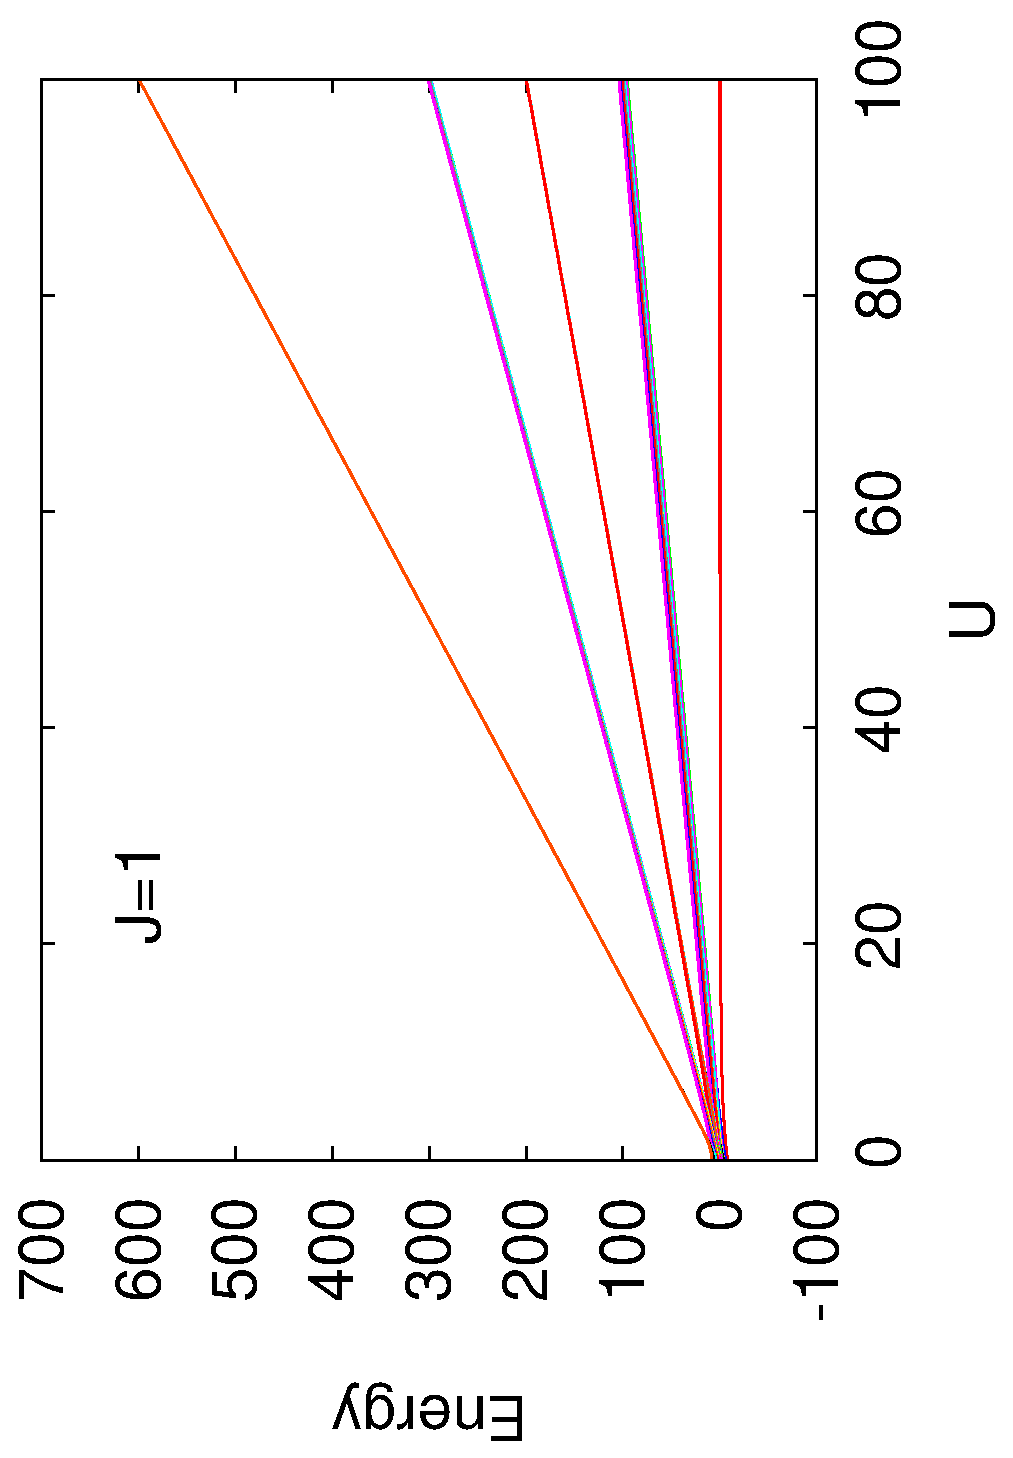
\includegraphics[width=0.35\textwidth, angle=270]{Long_Strong_NL4_NB4_J1.eps}}
  \subfloat[]{
   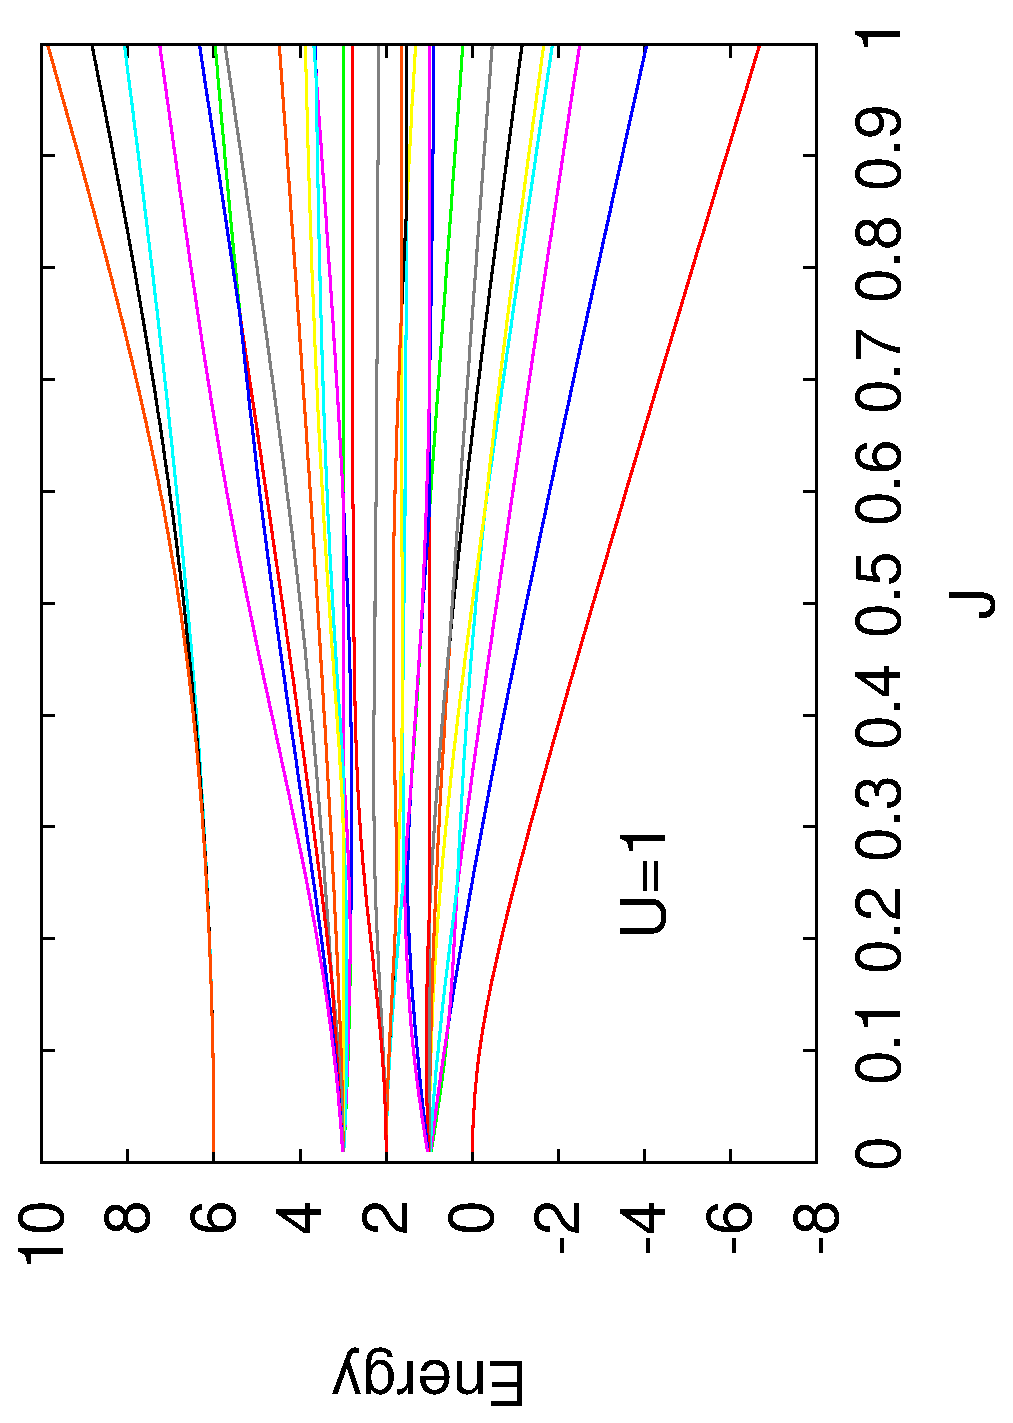
\includegraphics[width=0.35\textwidth, angle=270]{Short_Weak_NL4_NB4_U1.eps}}
  \caption{}
 \label{f:comparacion}
\end{figure}


 
Este tipo de redes son muy versátiles: se pueden conseguir muchas geometrías diferentes casi sin defectos, e incluso puede cambiarse su forma y la intensidad de los mínimos de potencial en el curso de un experimento. 




\end{document}
